\section*{Лабораторная работа №3\\ 
<<Параллельные вычисления в модели общей памяти.>>}

\subsection*{Цель работы}
Приобретение навыков: распараллеливания программ и оценки ускорения, эффективности и производительности параллельных алгоритмов в модели общей памяти.
Объектом исследования является исходный и исполняемый код программ, реализующих операции вычислительной линейной алгебры, отлича\-ющиеся арифметической сложностью и интенсивностью.

\subsection*{Задание}
\begin{enumerate}
\item Реализовать заданные алгоритмы на языке программирования C++ с использованием параллельных технологий программирования OpenMP.
\item Используя созданные программы определить время выполнения и программ при вычислениях на заданном числе процессорных ядер и потоков/процессов.
\item Оценить ускорение и эффективность параллельных вычислений, производительность программ, используя Roofline модель.
\end{enumerate}

\subsection*{Теоретическая часть}
Параллельные вычисления являются одним из основных инструментов получения высокой производительности вычислений, которая достигается распределением вычислений между вычислительными ресурсами: кластерами, модулями, процессорами, процессорными ядрами [1]. Взаимодействия параллельных потоков реализуются в рамках многопоточного программирования, использующего модель общей памяти (общего адресного пространства). 

Многопоточное программирование не обеспечивает взаимодействие параллельных процессов, когда данные находятся разных адресных пространствах. В этом случае, для взаимодействия параллельных процессов в основном применяется модель передачи сообщений. Многопоточное программирование реализуется и средствами языка, и в виде внешних библиотек, как, например, технология OpenMP [2], обеспечивающая межплатформенную переносимость исходного кода и его высокоуровневое (циклов) и низкоуровневое (циклов, блоков кода, функций) распараллеливание. 

Параллельные вычисления характеризуются понятиями ускорение и эффективность.

Ускорение $S_p$ параллельных вычислений определяется следующим образом:
\begin{equation}\label{eq31}
   S_p=\dfrac{T_1}{T_p},
\end{equation}                                                                        
где $T_1$ --- время выполнения одним процессом/потоком, $T_p$  ---  время выполнения $p$ процессами/потоками.

Эффективность $E_p$ определяется как отношение:
\begin{equation}\label{eq32}
   E_p=\dfrac{S_p}{p}\cdot 100\%,
\end{equation}                                                                        

Ускорение показывает во сколько раз параллельные вычисления выполнены быстрее последовательных, а эффективность — насколько при этом были задействованы вычислительные ресурсы, т. к.  полагается равным числу использованных процессоров или процессорных ядер.

Закон Амдала (1967 г.) описывает изменение ускорения параллельных вычислений при решении задачи фиксированного размера при увеличении числа используемых (ядер) процессоров:
\begin{equation}\label{eq33}
   S_p=\dfrac{1}{f+\dfrac{1-f}{p}}=\dfrac{p}{f\cdot(p-1)+1},
\end{equation}                                                                        
где $0\leqslant f\leqslant 1$ --- доля последовательных вычислений; $p$ --- число используемых (ядер) процессоров. Масштабирование времени в этом случае называется сильным.

Если размер задачи увеличивается пропорционально числу (ядер) процессоров, то ускорение изменяется согласно закону Густафсона--Барсиса (1988 г.):
\begin{equation}\label{eq34}
   S_p=p-f\cdot(p-1).
\end{equation}                                                                        
Как следствие, задача большего размера может быть решена за то же время с использованием большего числа (ядер) процессоров. Масштабирование времени в этом случае называется слабым.

Наиболее затратной частью программ, подвергающихся распараллеливанию, являются циклы [3,4]. Циклы применяются при поиске экстремальных значений в структурах данных, суммировании данных, в других операциях вычислительной линейной алгебры.
В технологии OpenMP реализовано несколько способов распараллеливания циклов: 
\begin{enumerate}
    \item <<Низкоуровневое>>, в котором итерации цикла разделяются в зависимости от номера потока; 
    \item С применением директивы \verb|#pragma omp for| внутри параллельной области или ее краткой формы \verb|#pragma omp parallel for|; 
    \item С применением \verb|#pragma omp sections| внутри параллельной области и ее краткой формы \verb|#pragma omp parallel sections|, но данный способ чаще применяется к распараллеливанию блоков программного кода. 
\end{enumerate}
В данной работе применяется второй способ распределения итераций циклов. В директиве \verb|#pragma omp for| может задаваться опция \verb|schedule(type,chunk)|, где \verb|type| --- порядок распределения итераций, а необязательный параметр \verb|chunk| --- число итераций, приходящихся на поток. Параметр \verb|type| может принимать значения \verb|static|, \verb|dynamic|, \verb|guided|, \verb|auto|, \verb|runtime| [2,4,6]. 

\subsection*{Практическая часть.}
Реализовать задания из Лабораторной работы №1, используя технологии параллельного программирования OpenMP для модели общей памяти:
\begin{enumerate}
\item Выполнить вычислительные эксперименты на кластере из миникомпьютеров.
\item Построить графики ускорения и эффективности в зависимости от числа вычислительных потоков/процессов. 
\item Построить графики зависимости производительности от арифметической интенсивности, ограниченные Roofline ломанной. 
\end{enumerate}
Рассмотреть случаи оптимизации исполняемого кода средствами компилятора (опции -O0,-O3).

\textbf{Аппаратное обеспечение работы:} кластер из миникомпьютеров.
Кластер состоит из 8 миникомпьютеров Raspeberry Pi 4 Model B Rev. 1.4, соединенных сетью Gigabit Ethernet. Каждый миникомпьютер оснащен 4-ядерным ARM процессором (ядра Cortex-A72 (ARM v8) с частотой 1,5 GHz) и 8 GB оперативной памяти LPDDR4-3200.

\textbf{Программное обеспечение:}
Операционная система 64-разрядная Ubuntu 20.04 LTS, компилятор GNU g++ 10.3.0, библиотеки Open MPI 4.0.3.

\subsection*{Практическая часть №1.}
На листинге~\ref{lst31} представлен фрагмент исходного кода на языке C++ с применением распараллеливания циклов в технологии OpenMP для параллельного вычисления 
\ifcase\Zadanie
$\gamma=(x,y), \; x,y\in\mathbb{R}^N, \gamma\in\mathbb{R},$ 
\or 
$y=\alpha x+y, \; x,y\in\mathbb{R}^N, \alpha\in\mathbb{R},$ 
\or 
$z=x+y, \; x,y,z\in\mathbb{R}^N,$ 
\or 
$y=\alpha x, \; x,y\in\mathbb{R}^N, \alpha\in\mathbb{R},$ 
\or 
$\gamma=\sum_{i=1}^{N}x_i, \; x\in\mathbb{R}^N, \gamma\in\mathbb{R},$
\fi
 обозначено (1). 

\lstinputlisting[language=C++, firstline=38, lastline=41, caption={Фрагмент кода на С++, реализующий (1) с применением OpenMP},label={lst31}]{Lab3/lab31.cpp} 


% для миникопьютера
\def\perfFirst{1.5*4}  % P_{max}  для Практической части №1
\def\bwFirst{6.4} % B  для Практической части №1
\def\icrossFirst{\perfFirst/\bwFirst} % I_* =P_{max}/B  для Практической части №1
% для кластера
\def\perfSecond{1.5*32} % P_{max}  для Практической части №2
\def\bwSecond{0.125} % B  для Практической части №2
\def\icrossSecond{\perfSecond/\bwSecond} % I_*=P_{max}/B для Практической части №2

\begin{figure}[H]
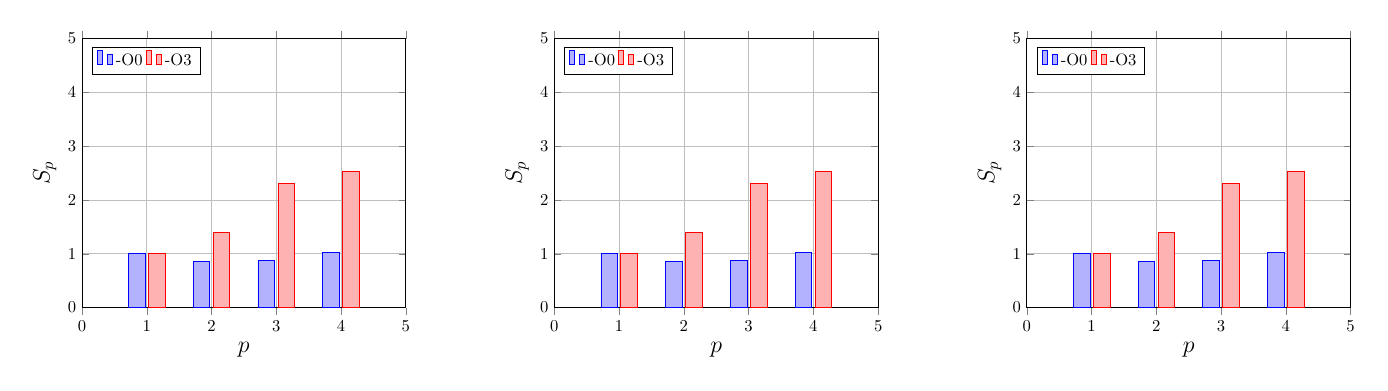
\begin{tikzpicture}
\begin{scope}[scale=0.6]
\begin{axis}[
 ybar,
 xmin=0, ymin=0,
 ymax=5,  xmax=5, %32
 xlabel={\Large $p$}, ylabel={\Large $S_p$},
 grid=major,
legend columns=-1,
legend pos= north west,
tick=empty
]
\addplot coordinates {(1,1) (2, 0.863) (3, 0.869) (4, 1.02)};
\addlegendentry{-O0}
\addplot coordinates {(1,1) (2, 1.4) (3, 2.3) (4, 2.53)};
\addlegendentry{-O3}
\end{axis}
\end{scope}

\begin{scope}[xshift=6cm,scale=0.6]
\begin{axis}[
 ybar,
 xmin=0, ymin=0,
 ymax=5,  xmax=5, %32
 xlabel={\Large $p$}, ylabel={\Large $S_p$},
 grid=major,
legend columns=-1,
legend pos= north west,
tick=empty
]
\addplot coordinates {(1,1) (2, 0.863) (3, 0.869) (4, 1.02)};
\addlegendentry{-O0}
\addplot coordinates {(1,1) (2, 1.4) (3, 2.3) (4, 2.53)};
\addlegendentry{-O3}
\end{axis}
\end{scope}
\begin{scope}[xshift=12cm,scale=0.6]
\begin{axis}[
 ybar,
 xmin=0, ymin=0,
 ymax=5,  xmax=5, %32
 xlabel={\Large $p$}, ylabel={\Large $S_p$},
 grid=major,
legend columns=-1,
legend pos= north west,
tick=empty
]
\addplot coordinates {(1,1) (2, 0.863) (3, 0.869) (4, 1.02)};
\addlegendentry{-O0}
\addplot coordinates {(1,1) (2, 1.4) (3, 2.3) (4, 2.53)};
\addlegendentry{-O3}
\end{axis}
\end{scope}
\end{tikzpicture}
\caption{Ускорение $S_p(p)$ параллельных вычислений, технология OpenMP,\\ \mbox{\hspace{2.5cm}}при $N\in\{32000, 3200000, 32000000\}$}
    \label{fig31:Sp}
\end{figure}

\begin{figure}[H]
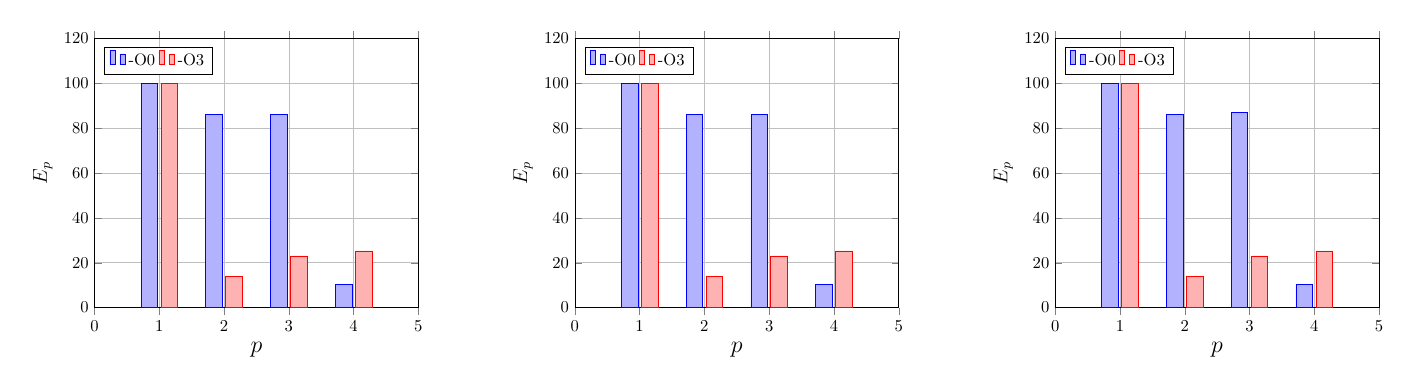
\begin{tikzpicture}
\begin{scope}[scale=0.6]
\begin{axis}[
 ybar,
 xmin=0, ymin=0,
 ymax=120,  xmax=5, %32
 xlabel={\Large $p$}, ylabel={\large $E_p$},
 grid=major,
legend columns=-1,
legend pos= north west,
tick=empty
]
\addplot coordinates {(1,100) (2, 86.3) (3, 86) (4, 10.2)};
\addlegendentry{-O0}
\addplot coordinates {(1,100) (2, 14.) (3, 23.) (4, 25.3)};
\addlegendentry{-O3}
\end{axis}
\end{scope}
\begin{scope}[xshift=6.1cm,scale=0.6]
\begin{axis}[
 ybar,
 xmin=0, ymin=0,
 ymax=120,  xmax=5, %32
 xlabel={\Large $p$}, ylabel={\large $E_p$},
 grid=major,
legend columns=-1,
legend pos= north west,
tick=empty
]
\addplot coordinates {(1,100) (2, 86.) (3, 86.) (4, 10.2)};
\addlegendentry{-O0}
\addplot coordinates {(1,100) (2, 14.) (3, 23.) (4, 25.3)};
\addlegendentry{-O3}
\end{axis}
\end{scope}
\begin{scope}[xshift=12.2cm,scale=0.6]
\begin{axis}[
 ybar,
 xmin=0, ymin=0,
 ymax=120,  xmax=5, %32
 xlabel={\Large $p$}, ylabel={\large $E_p$},
 grid=major,
legend columns=-1,
legend pos= north west,
tick=empty
]
\addplot coordinates {(1,100) (2, 86.3) (3, 86.9) (4, 10.2)};
\addlegendentry{-O0}
\addplot coordinates {(1,100) (2, 14.) (3, 23.) (4, 25.3)};
\addlegendentry{-O3}
\end{axis}
\end{scope}
\end{tikzpicture}
\caption{Эффективность $E_p(p)$ параллельных вычислений,~\%, технология OpenMP\\
\mbox{\hspace{2.5cm}}при $N\in\{32000, 3200000, 32000000\}$}
    \label{fig31:Ep}
\end{figure}

\begin{figure}[H]
    \centering
\begin{tikzpicture}

\begin{loglogaxis}[
    axis lines = left,
    xlabel = {$I$, FLOP/byte},
    ylabel = {$P$, GFLOP/s}, 
    legend pos = south east
]

\addplot [
    domain=0.001:10000, 
    samples=200, 
    color=black,
    dashed
    ]
    {x <= \icrossFirst ?  \bwFirst *x : \perfFirst}; % (2)
    \addlegendentry{RPi4}

\addplot [
    domain=0.001:10000, 
    samples=200, 
    color=black
    ]
    {x <= \icrossSecond ?  \bwSecond *x : \perfSecond}; % (2)
    \addlegendentry{кластер}

\addplot [only marks, color=black, mark=square] coordinates {
    (0.083, 0.293)
    };
\addlegendentry{(1) OpenMP}

\addplot [only marks, color=black, mark=square*, mark color=black] coordinates {
    (114.28, 0.44) 
    };
\addlegendentry{(2) OpenMP}

\end{loglogaxis}
\end{tikzpicture}
    \caption{Производительность параллельных вычислений для заданий (1) и (2) с применением технологии OpenMP, и Roofline модели кластера и миникомпьютера (RPi4).}
    \label{fig:RL3}
\end{figure}


\subsection*{Практическая часть №2.}
На листинге~\ref{lst32} представлен фрагмент исходного кода на языке C++ с применением распараллеливания циклов в технологии OpenMP для параллельного вычисления $C=A\cdot B$ в виде <<ijk>>, обозначено (2), где $A\in \mathbb{R}^{M\times N}$, $B\in \mathbb{R}^{N\times M}$, $C\in \mathbb{R}^{M\times M}$.

\lstinputlisting[language=C++, firstline=97, lastline=116, caption={Фрагмент кода на С++, реализующий (2) с применением OpenMP},label={lst32}]{Lab3/lab32.cpp} 

\begin{figure}[H]
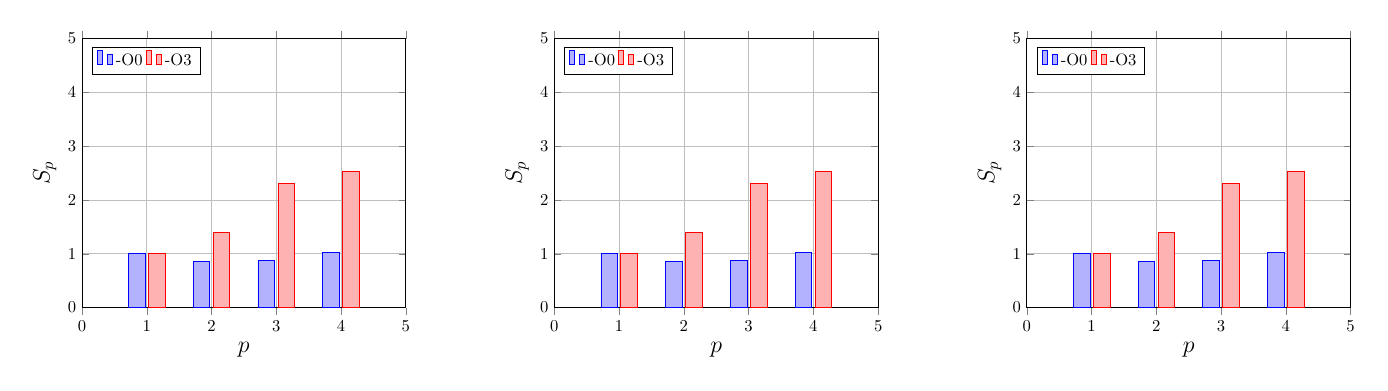
\begin{tikzpicture}
\begin{scope}[scale=0.6]
\begin{axis}[
 ybar,
 xmin=0, ymin=0,
 ymax=5,  xmax=5, %32
 xlabel={\Large $p$}, ylabel={\Large $S_p$},
 grid=major,
legend columns=-1,
legend pos= north west,
tick=empty
]
\addplot coordinates {(1,1) (2, 0.863) (3, 0.869) (4, 1.02)};
\addlegendentry{-O0}
\addplot coordinates {(1,1) (2, 1.4) (3, 2.3) (4, 2.53)};
\addlegendentry{-O3}
\end{axis}
\end{scope}

\begin{scope}[xshift=6cm,scale=0.6]
\begin{axis}[
 ybar,
 xmin=0, ymin=0,
 ymax=5,  xmax=5, %32
 xlabel={\Large $p$}, ylabel={\Large $S_p$},
 grid=major,
legend columns=-1,
legend pos= north west,
tick=empty
]
\addplot coordinates {(1,1) (2, 0.863) (3, 0.869) (4, 1.02)};
\addlegendentry{-O0}
\addplot coordinates {(1,1) (2, 1.4) (3, 2.3) (4, 2.53)};
\addlegendentry{-O3}
\end{axis}
\end{scope}
\begin{scope}[xshift=12cm,scale=0.6]
\begin{axis}[
 ybar,
 xmin=0, ymin=0,
 ymax=5,  xmax=5, %32
 xlabel={\Large $p$}, ylabel={\Large $S_p$},
 grid=major,
legend columns=-1,
legend pos= north west,
tick=empty
]
\addplot coordinates {(1,1) (2, 0.863) (3, 0.869) (4, 1.02)};
\addlegendentry{-O0}
\addplot coordinates {(1,1) (2, 1.4) (3, 2.3) (4, 2.53)};
\addlegendentry{-O3}
\end{axis}
\end{scope}
\end{tikzpicture}
\caption{Ускорение $S_p(p)$ параллельных вычислений, технология OpenMP,\\ 
\mbox{\hspace{2.5cm}}при $N\times N \in \{320\times 320, 640\times 640, 1280\times 1280\}$}
    \label{fig32:Sp}
\end{figure}

\begin{figure}[H]
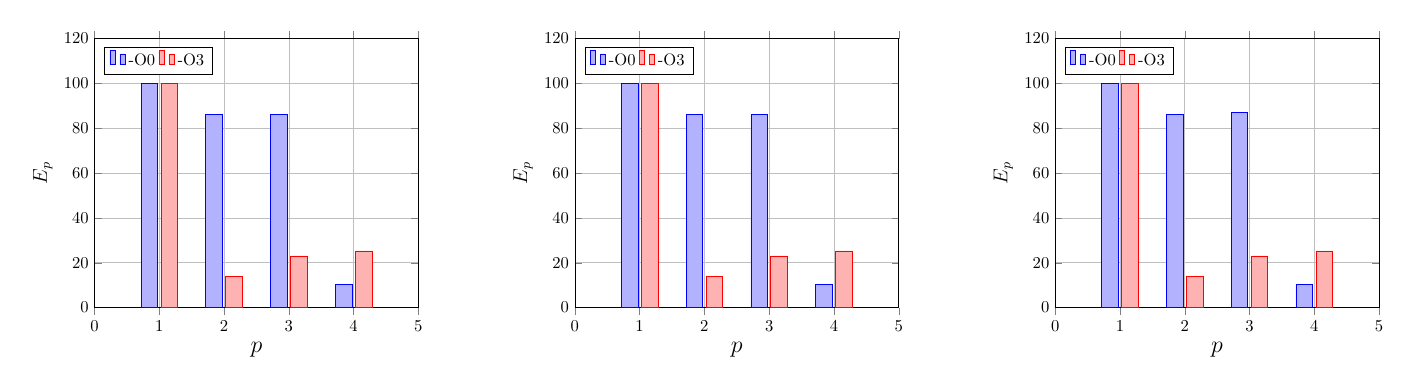
\begin{tikzpicture}
\begin{scope}[scale=0.6]
\begin{axis}[
 ybar,
 xmin=0, ymin=0,
 ymax=120,  xmax=5, %32
 xlabel={\Large $p$}, ylabel={\large $E_p$},
 grid=major,
legend columns=-1,
legend pos= north west,
tick=empty
]
\addplot coordinates {(1,100) (2, 86.3) (3, 86) (4, 10.2)};
\addlegendentry{-O0}
\addplot coordinates {(1,100) (2, 14.) (3, 23.) (4, 25.3)};
\addlegendentry{-O3}
\end{axis}
\end{scope}
\begin{scope}[xshift=6.1cm,scale=0.6]
\begin{axis}[
 ybar,
 xmin=0, ymin=0,
 ymax=120,  xmax=5, %32
 xlabel={\Large $p$}, ylabel={\large $E_p$},
 grid=major,
legend columns=-1,
legend pos= north west,
tick=empty
]
\addplot coordinates {(1,100) (2, 86.) (3, 86.) (4, 10.2)};
\addlegendentry{-O0}
\addplot coordinates {(1,100) (2, 14.) (3, 23.) (4, 25.3)};
\addlegendentry{-O3}
\end{axis}
\end{scope}
\begin{scope}[xshift=12.2cm,scale=0.6]
\begin{axis}[
 ybar,
 xmin=0, ymin=0,
 ymax=120,  xmax=5, %32
 xlabel={\Large $p$}, ylabel={\large $E_p$},
 grid=major,
legend columns=-1,
legend pos= north west,
tick=empty
]
\addplot coordinates {(1,100) (2, 86.3) (3, 86.9) (4, 10.2)};
\addlegendentry{-O0}
\addplot coordinates {(1,100) (2, 14.) (3, 23.) (4, 25.3)};
\addlegendentry{-O3}
\end{axis}
\end{scope}
\end{tikzpicture}
\caption{Эффективность $E_p(p)$ параллельных вычислений,~\%, технология OpenMP\\
\mbox{\hspace{2.5cm}}при $N\times N \in \{320\times 320, 640\times 640, 1280\times 1280\}$}
    \label{fig32:Ep}
\end{figure}

\input{Lab3/pic32RL}

\newpage
\subsection*{Выводы}
\begin{enumerate}
\item По результатам вычислительных экспериментов на кластере из миникомпьютеров \\Raspeberry Pi 4, определены ускорение и эффективность параллельного вычисления (1) для векторов размерности 32000, 3200000, 32000000 и %одинарная 
(2) --- произведения двух вещественных матриц размеров $320\times 320$, $640\times 640$, $1280\times 1280$, определена производительность. 
\item Максимальные ускорения и эффективность составили: 2.53 и 76.8\%
 для 4 и 3 вычислительных потоков при распараллеливании циклов в технологии OpenMP при размере матрицы $1280\times 1280$. 
%Сверхлинейное ускорение, как правило, объясняется тем, что данные в параллельном случае выравнены лучше и обрабатываются с меньшим числом промахов кэша.
\item Получены максимальные значения производительности, в случае применения OpenMP:  0.44 GFLOP/s, пиковая производительность кластера при вычислениях с одинарной точностью составляет 96 GFLOP/s (8 миникомпьютеров, по 4х-ядерному процессору в каждом, тактовая частота 1.5 ГГц и 2 арифметических операции с плавающей точкой за цикл).
\end{enumerate}

\subsection*{Список литературы}
1.~Копысов С.П., Новиков А.К. Промежуточное программное обеспечение параллельных вычислений. --- Ижевск: Изд-во «Удмуртский университет». 2012. --- 140 с.\\
2.~OpenMP. [Электронный ресурс]. URL: \url{https://www.openmp.org}. 
 Дата обращения 21.03.2023.\\
3.~Ортега Дж. Введение в параллельные и векторные методы решения линейных систем. --- М.: «Мир». 1991. --- 367 с.\\ 
4.~Малявко А.А. Параллельное программирование на основе технологий OpenMP, CUDA, OpenCL, MPI: учеб. пособие для вузов. --- М.: Изд-во Юрайт, 2022. --- 135 с.\\ 
5.~Копысов С. П., Кузьмин И. М., Недожогин Н. С. Масштабируемые вычисления для гетерогенных платформ: учебное пособие. --- Ижевск: Издательский центр «Удмуртский университет», 2020. --- 272 с.\\ 
6.~Антонов А.С. Параллельное программирование с использованием технологии OpenMP: учебное пособие. --- М.: Изд-во МГУ, 2009. --- 77 с.
